\section{Filesystems}
\subsection{Unix filesystems}
A Unix filesystem uses a data structure called an \textit{inode}. The inodes are found in an inode table and each inode keeps track of the size, blocks used for the file's data, and metadata for the files in the filesystem, and a directory simply contains the file names and each file or directory's inode id. The system can with an inode id find information about the file or directory using the inode table. Each inode can contain any metadata that might be relevant for the system, such as creation time and last update time. 

Figure~\ref{fig:inode_diag} shows how example inode filesystem and how it can be visualized. The blocks of an inode entry is where in the storage device the data is stored, each block is often defines as a certain amount of bytes. Listing~\ref{lst:inode_fs} describes a simple implementation of an inode, an inode table, and directory entries. 

 % TODO: Add info about how FFS will only implement some metadata? And/or add that to delimitations too

\begin{figure}[!ht]
	\begin{center}
	  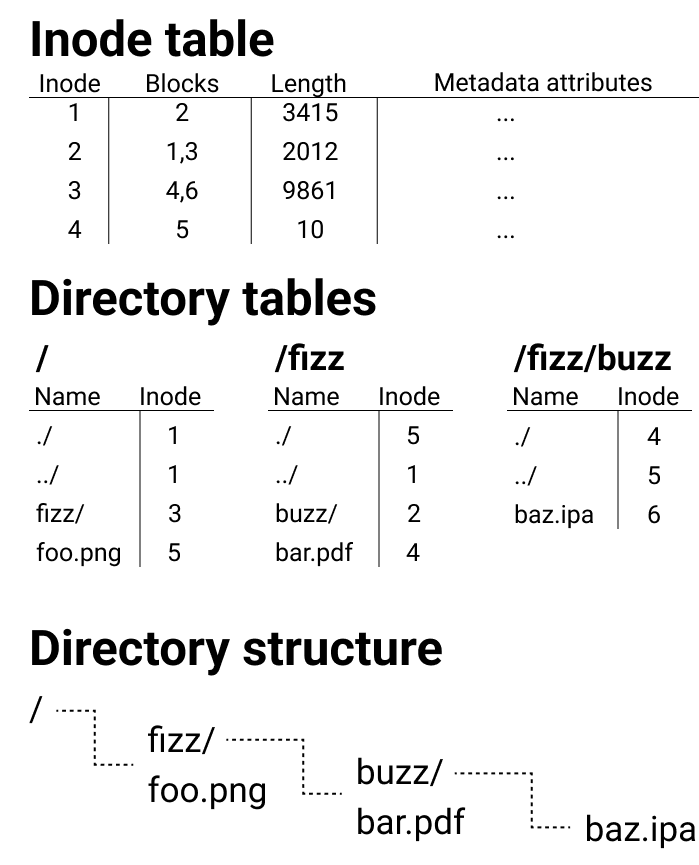
\includegraphics[width=0.5\textwidth]{figures/inode_diagram.png}
	\end{center}
	\caption{Basic structure of inode based filesystem}
	\label{fig:inode_diag}
\end{figure}

\begin{minipage}{\linewidth}
\begin{lstlisting}[language=c, caption={Pseudocode of a minimalistic inode filesystem structure}, label=lst:inode_fs]
struct inode_entry {
	int 	length
	int[]	blocks
	// Metadata attributes are defined here
}

struct directory_entry {
	char*   filename
	int     inode
}

// Maps inode_id to a inode_entry
map<int, inode_entry> inode_table

\end{lstlisting}
\end{minipage}

Different filesystems provide different features and limitations. Extended Filesystem (ext) exist in four different versions; ext, ext2, ext3, and ext4, and is often used on Unix systems. Each iteration brings new features and changes the limitations. For instance, comparing the two latest iterations, ext3 and ext4, ext4 can theoretically store files up to \SI{16}{\tebi\byte} while ext3 can store files up to \SI{2}{\tebi\byte}\cite{salterUnderstandingLinuxFilesystems2018}. ext4 also support timestamps at nanoseconds while et3 only support timestamp down to the second. The Zettabyte filesystem (ZFS) introduces features that no version of ext supports, such as block-level cryptographic checksumming.

\subsection{Distributed filesystems}
Filesystems are used to store data on for instance a hard drive of a computer locally or in the cloud. For example, Google Drive is a filesystem that enables users to save their data online with up to 15 GB for free\cite{CloudStorageWork} using their clusters of distributed storage devices, meaning that the data is saved on their servers which can be located wherever they have data centers\cite{DistributedStorageWhat}. Paying customers can have a greater amount of storage using the service. Apple's iCloud and Microsoft's OneDrive are two additional examples of distributed filesystems where users have the option of free-tier and paid-tier storage.

\subsection{Image structures}
Different file types have different protocols and definitions of how they should be encoded and decoded, for instance a JPEG and a PNG file can be used to display similar content but the data they store is different. At the lowest level, storage devices often represent files as a string of binary digits no matter the file type (however there are non-binary storage devices too\cite{MultistateDataStorage2020}). If one would represent an arbitrary file of $X$ bytes, each byte (0x00 - 0xFF) can be represented as a character such as the Extended ASCII (EASCII) keyset and we can therefore decode this file as $X$ different characters. Using the same set of characters for encoding and decoding we can get a symmetric relation for representing a file as a string of characters. EASCII is only one example of such a set of characters, any set of strings with 256 unique symbols can be used to create such a symmetric relation, for instance 256 different emojis or a list of 256 different words. However, if we are using a set of words we must also introduce a unique separator so that the words can be distinguished. If we would use a single space character as the separator, we could make the encoded text look like an actual text document, however with random words after another with high probability of creating unstructured sentences.

This string of $X$ bytes can also be used as the data in an image. An image can be abstracted as a $h * w$ matrix, where each element is a pixel of a certain color. In an image with 8-bit RGB color depth, each pixel consist of three 8-bit values, i.e. three bytes. One can therefore imagine that we can use this string of $X$ bytes to assign colors in this pixel matrix by assigning the first three bytes as the first pixel's color, the next three bytes as the following pixel's color and so forth. This means that $X$ bytes of data can be represented as 
$$ceil(\frac{X}{3})$$ 
pixels, where $ceil$ rounds a float to the closest larger integer. For a file of \SI{1}{\mega\byte}, i.e. $X = 1\,000\,000$ we need $333\,334$ pixels. The values of $h$ and $w$ are arbitrary but if we for instance want a square image we can set $ h\,=\,w\,=\,578$ which means that there will be $334\,084$ pixels in total, and the remaining $750$ pixels will just be fillers to make the image a reasonable size. However, we could choose $h = 1$ and $w = 333\,334$ which would mean a very wide image but would not require filler pixels. 

This means that we can represent any file as a string of text or as an image, which can be posted on for instance social media. 
